% Provenance (never printed): cycle 4 SVT, "La planete Terre": volcanic
% activity, its products and its link with plate boundaries; natural hazards
% and their monitoring; see sources/book1/PROVENANCE.md. Book 1, grade 7,
% chapter 2.
% Vocabulary guard: "magma" first allowed here; "sediment" not before g7.4;
% "subduction zone" is never a term here (gloss: "where one plate sinks under
% another"); "hotspot track" is Book 2's; lahars are called mudflows.
\chapter{Vulkanen}\label{ch:g7:volcanoes}

Op 17~mei 1980 stond een geoloog op een bergkam tien kilometer van Mount
St.~Helens, in het noordwesten van de Verenigde Staten, en maakte hij de
foto hieronder links: een gladde, besneeuwde kegel, een van de sierlijkste
\omterm{def:g1:landscapes-around-us:landform}{bergen} van het land. Al twee maanden trilde de \omterm{def:g1:landscapes-around-us:landform}{berg}, en zijn noordflank
zwol als een ballon naar buiten op. De volgende ochtend, om 8.32~uur,
schudde een kleine \omterm{def:g4:volcanoes-earthquakes-first-look:earthquake}{aardbeving} hem door elkaar. De hele opgezwollen flank
gleed weg, en de \omterm{def:g4:volcanoes-earthquakes-first-look:volcano}{vulkaan} explodeerde zijwaarts. Toen dezelfde bergkam in
september weer gefotografeerd kon worden, zag de \omterm{def:g1:landscapes-around-us:landform}{berg} eruit als op de foto
rechts.

\begin{omfigure}
\begin{minipage}[b]{0.495\linewidth}\centering
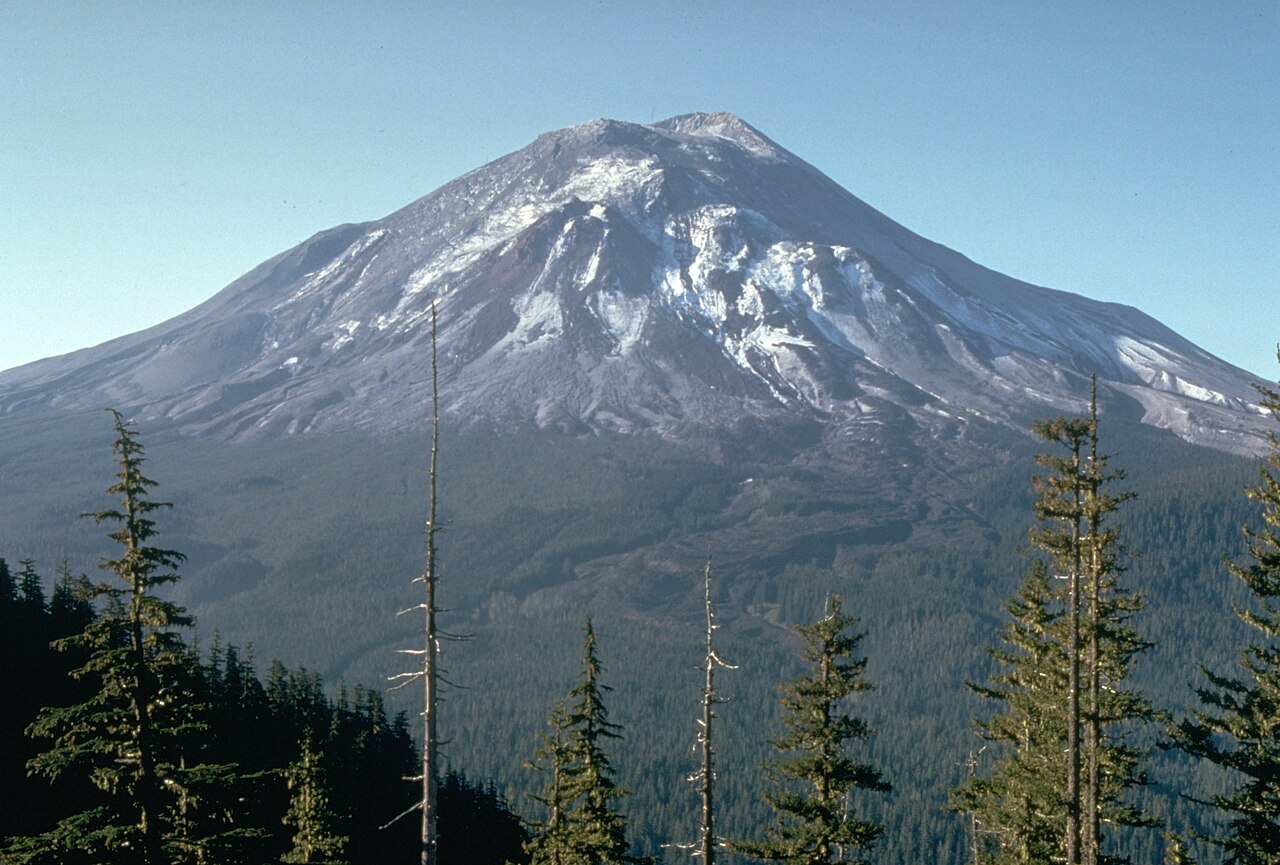
\includegraphics[width=\linewidth]{images/book1/g7-msh-before.jpg}

{\small 17 mei 1980, de dag ervoor.}
\end{minipage}\hfill
\begin{minipage}[b]{0.495\linewidth}\centering
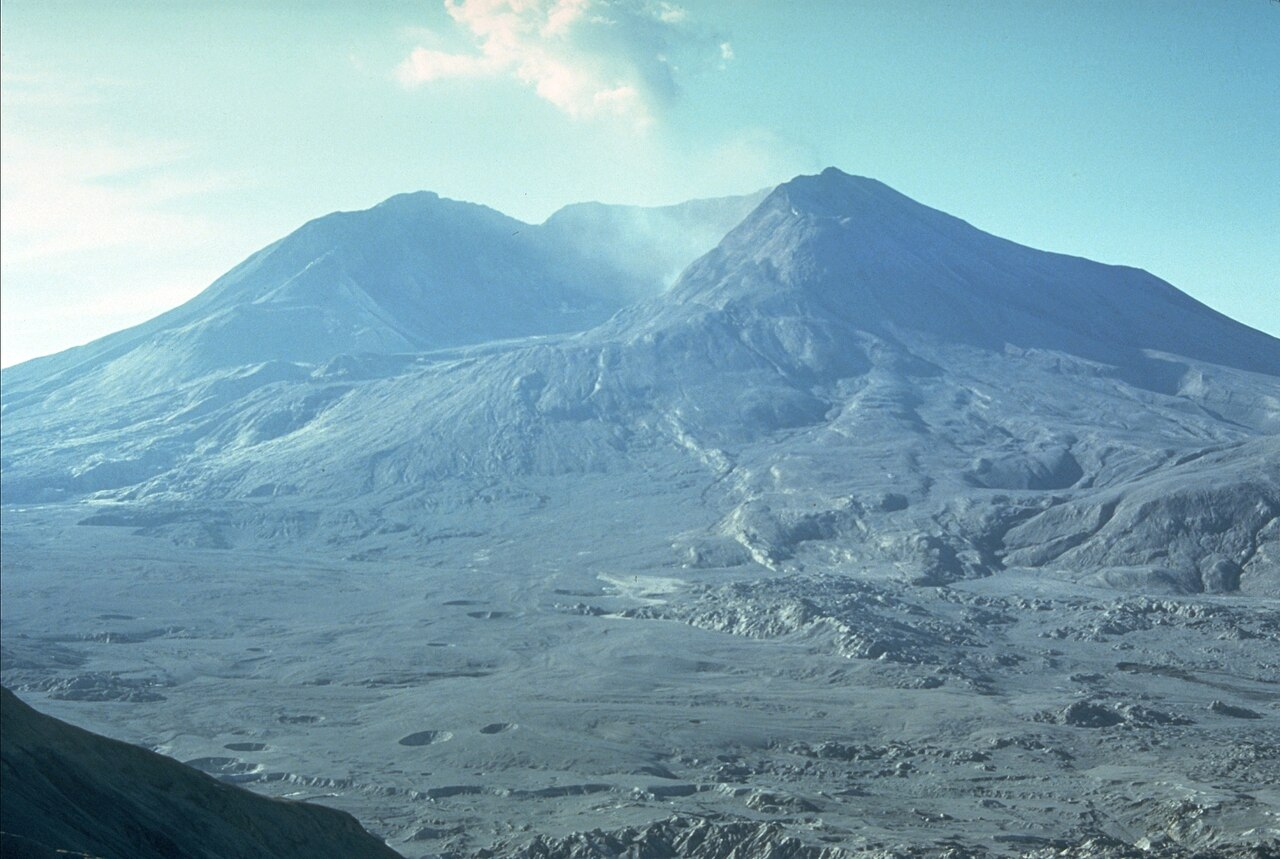
\includegraphics[width=\linewidth]{images/book1/g7-msh-after.jpg}

{\small 10 september 1980.}
\end{minipage}

{\small Mount St.~Helens gezien vanaf Johnston Ridge, voor en na de
\omterm{def:g4:volcanoes-earthquakes-first-look:eruption}{uitbarsting} van 18~mei 1980. De top en de hele noordflank zijn verdwenen;
een \omterm{def:g7:volcanoes:vent}{krater} die naar het noorden openstaat, heeft hun plaats ingenomen.
Foto's: Harry Glicken, U.S. Geological Survey (publiek domein, via
Wikimedia Commons).}
% ledger: commons:msh-before, commons:msh-after, usgs:msh-lead-up, usgs:msh-may18
\label{fig:g7:volcanoes:st-helens}
\end{omfigure}

In dit hoofdstuk snijden we een \omterm{def:g4:volcanoes-earthquakes-first-look:volcano}{vulkaan} open om te zien wat een
\omterm{def:g4:volcanoes-earthquakes-first-look:eruption}{uitbarsting} aandrijft; we ontdekken waarom sommige \omterm{def:g4:volcanoes-earthquakes-first-look:volcano}{vulkanen} rustige \omterm{def:g1:landscapes-around-us:water}{rivieren}
van \omterm{def:g4:volcanoes-earthquakes-first-look:eruption}{lava} uitstorten terwijl andere zichzelf opblazen; en we bekijken de
\omterm{def:g3:continents-and-oceans:world-map}{wereldkaart} opnieuw om te zien waar de \omterm{def:g4:volcanoes-earthquakes-first-look:volcano}{vulkanen} liggen, en waarom.

\begin{recall}
Een \emph{\omterm{def:g4:volcanoes-earthquakes-first-look:volcano}{vulkaan}} is een plek waar gesmolten \omterm{def:g3:stones-pebbles-sand:rock}{gesteente} van diep in de
Aarde aan het oppervlak komt, en de \omterm{def:g1:landscapes-around-us:landform}{heuvel} of \omterm{def:g1:landscapes-around-us:landform}{berg} die het daar opbouwt.
Tijdens een \emph{\omterm{def:g4:volcanoes-earthquakes-first-look:eruption}{uitbarsting}} stoot hij \omterm{def:g4:volcanoes-earthquakes-first-look:eruption}{lava}, as en gas uit
(\cref{ch:g4:volcanoes-earthquakes-first-look}). Onder de \omterm{def:g6:inside-the-earth:layers}{aardkorst} bestaat
de \omterm{def:g6:inside-the-earth:layers}{mantel} uit heet \omterm{def:g3:stones-pebbles-sand:rock}{gesteente} dat vast is, hoewel het heel langzaam kan
kruipen (\cref{ch:g6:inside-the-earth}). Basalt en graniet zijn
\omterm{def:g6:rocks-and-minerals:rock-families}{stollingsgesteenten}: ze ontstaan als gesmolten \omterm{def:g3:stones-pebbles-sand:rock}{gesteente} afkoelt en hard
wordt (\cref{ch:g6:rocks-and-minerals}). De buitenste schil van de Aarde is
gebroken in \omterm{def:g7:plate-tectonics:plate}{platen} die een paar centimeter per jaar bewegen; hun randen zijn
de \omterm{def:g7:plate-tectonics:plate-boundary}{plaatgrenzen} (\cref{ch:g7:plate-tectonics}).
\end{recall}

\section{In een vulkaan}

De \omterm{def:g6:inside-the-earth:layers}{mantel} is vast. Toch smelt op een paar plaatsen, diep onder het
oppervlak, een klein deel van het \omterm{def:g3:stones-pebbles-sand:rock}{gesteente}. Het gesmolten \omterm{def:g3:stones-pebbles-sand:rock}{gesteente} is
lichter dan het \omterm{def:g3:stones-pebbles-sand:rock}{vaste gesteente} eromheen, dus stijgt het langzaam op en
perst het zich door spleten omhoog, zoals een druppel olie die door water
opstijgt.
% ledger: usgs:hawaii-hotspot (magma lighter than the surrounding rock, rises)

\begin{definition}[Magma]\label{def:g7:volcanoes:magma}
\emph{Magma}\index{magma} is gesmolten \omterm{def:g3:stones-pebbles-sand:rock}{gesteente} onder de grond. Het is een
hete vloeistof die ook kristallen kan meevoeren en waarin gassen zijn
opgelost, zoals waterdamp en koolstofdioxide. Magma dat aan het oppervlak
komt, heet \omterm{def:g4:volcanoes-earthquakes-first-look:eruption}{lava}; bij het naar buiten komen verliest het het grootste deel
van zijn gas.
\end{definition}

Opstijgend \omterm{def:g7:volcanoes:magma}{magma} blijft onderweg vaak steken, een paar kilometer onder het
oppervlak, waar het zich verzamelt in een grote holte. Daar wacht het,
soms eeuwenlang, voordat een \omterm{def:g4:volcanoes-earthquakes-first-look:eruption}{uitbarsting} die holte gedeeltelijk leegmaakt.

\begin{definition}[Magmakamer]\label{def:g7:volcanoes:magma-chamber}
Een \emph{magmakamer}\index{magmakamer} is een grote ruimte in het \omterm{def:g3:stones-pebbles-sand:rock}{gesteente}
onder een \omterm{def:g4:volcanoes-earthquakes-first-look:volcano}{vulkaan}, een paar kilometer diep, waar \omterm{def:g7:volcanoes:magma}{magma} zich verzamelt voor
een \omterm{def:g4:volcanoes-earthquakes-first-look:eruption}{uitbarsting}.
\end{definition}

\begin{definition}[Eruptieopening en krater]\label{def:g7:volcanoes:vent}
Een \emph{eruptieopening}\index{eruptieopening} is een opening aan het
oppervlak waardoor \omterm{def:g7:volcanoes:magma}{magma}, gas en as naar buiten komen. Een
\emph{krater}\index{krater} is de komvormige holte rond een eruptieopening,
meestal op de top van de \omterm{def:g4:volcanoes-earthquakes-first-look:volcano}{vulkaan}.
\end{definition}

\begin{omfigure}
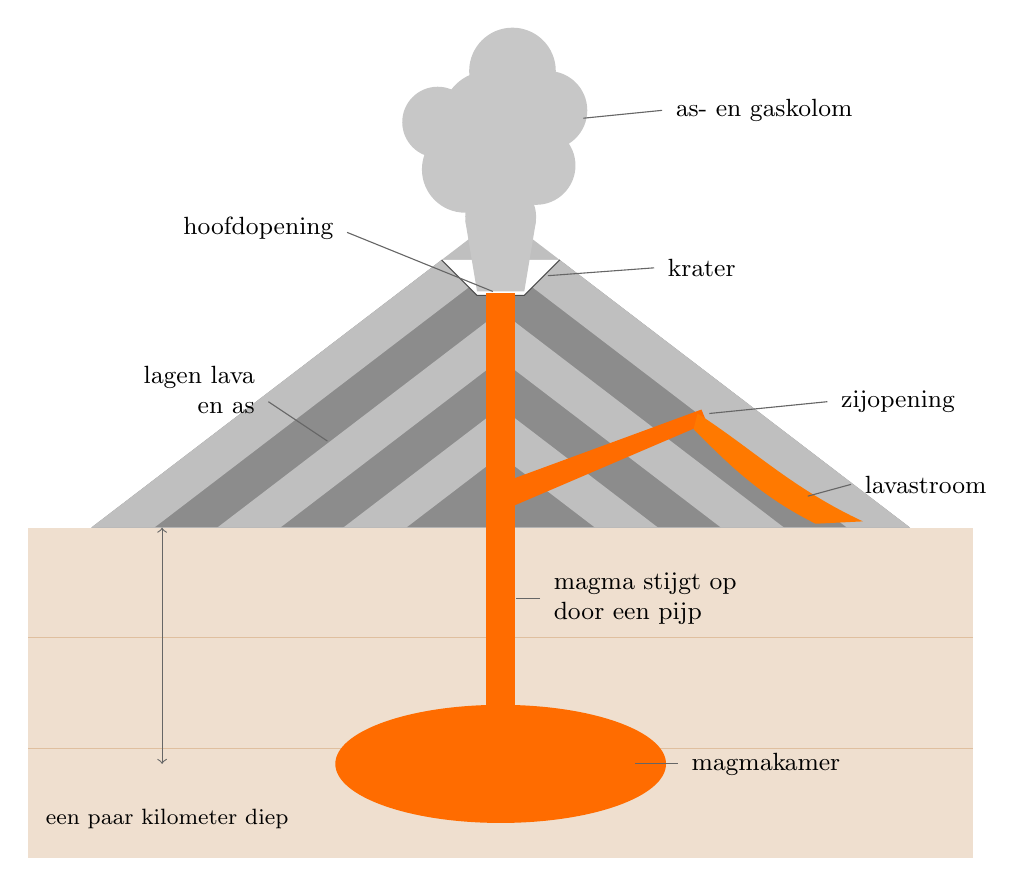
\begin{tikzpicture}[font=\small, x=1cm, y=1cm]
  % rocks below the volcano
  \fill[brown!25] (-6,-4.2) rectangle (6,0);
  \draw[brown!50] (-6,-1.4) -- (6,-1.4) (-6,-2.8) -- (6,-2.8);
  % the cone, built of layers of lava (dark) and ash (light)
  \fill[black!45] (-5.2,0) -- (-0.75,3.4) -- (0.75,3.4) -- (5.2,0) -- cycle;
    % layers dipping outwards, parallel to the flanks (slope 3.4/4.45)
  \foreach \k/\c in {0/black!25, 2/black!25, 4/black!25} {
    \pgfmathsetmacro{\xa}{-5.2+0.8*\k}\pgfmathsetmacro{\xb}{-5.2+0.8*(\k+1)}
    \pgfmathsetmacro{\ya}{(-0.18-\xa)*3.4/4.45}\pgfmathsetmacro{\yb}{(-0.18-\xb)*3.4/4.45}
    \fill[\c] (\xa,0) -- (-0.18,\ya) -- (-0.18,\yb) -- (\xb,0) -- cycle;
    \fill[\c] (-\xa,0) -- (0.18,\ya) -- (0.18,\yb) -- (-\xb,0) -- cycle;
  }
  % the crater at the top
  \fill[white] (-0.75,3.4) -- (-0.3,2.95) -- (0.3,2.95) -- (0.75,3.4) -- cycle;
  \draw[black!70] (-0.75,3.4) -- (-0.3,2.95) -- (0.3,2.95) -- (0.75,3.4);
  % magma chamber and the pipe up to the vent
  \fill[orange!85!red] (0,-3.0) ellipse (2.1 and 0.75);
  \fill[orange!85!red] (-0.18,-2.4) rectangle (0.18,2.98);
  % a side branch to a small side vent
  \fill[orange!85!red] (0.1,0.6) -- (2.55,1.5) -- (2.62,1.33) -- (0.1,0.25) -- cycle;
  % lava flow down the right flank, from the side vent
  \fill[orange!95!red] (2.5,1.45) .. controls (3.2,1.0) and (3.7,0.5) .. (4.6,0.08)
    -- (4.0,0.05) .. controls (3.3,0.4) and (2.9,0.8) .. (2.45,1.25) -- cycle;
  % ash column and gas
    \fill[black!22] (-0.3,3.0) -- (0.3,3.0) -- (0.45,3.9) -- (-0.45,3.9) -- cycle;
  \foreach \x/\y/\r in {0/3.95/0.45, -0.45/4.55/0.55, 0.45/4.6/0.5, -0.15/5.2/0.6,
                        0.6/5.3/0.5, -0.8/5.15/0.45, 0.15/5.8/0.55}
    \fill[black!22] (\x,\y) circle (\r);
  % labels
  \node[anchor=west] at (2.1,5.3) {as- en gaskolom};
  \draw[black!60] (2.05,5.3) -- (1.05,5.2);
  \node[anchor=west] at (2.0,3.3) {krater};
  \draw[black!60] (1.95,3.3) -- (0.6,3.2);
  \node[anchor=east] at (-2.0,3.8) {hoofdopening};
  \draw[black!60] (-1.95,3.75) -- (-0.1,3.0);
  \node[anchor=west] at (4.2,1.6) {zijopening};
  \draw[black!60] (4.15,1.6) -- (2.65,1.45);
  \node[anchor=west] at (4.5,0.55) {lavastroom};
  \draw[black!60] (4.45,0.55) -- (3.9,0.4);
  \node[anchor=east, align=right] at (-3.0,1.75) {lagen lava\\en as};
  \draw[black!60] (-2.95,1.6) -- (-2.2,1.1);
  \node[anchor=west, align=left] at (0.55,-0.9) {magma stijgt op\\door een pijp};
  \draw[black!60] (0.5,-0.9) -- (0.2,-0.9);
  \node[anchor=west] at (2.3,-3.0) {magmakamer};
  \draw[black!60] (2.25,-3.0) -- (1.7,-3.0);
  \node[anchor=west, align=left, font=\footnotesize] at (-5.9,-3.7) {een paar kilometer diep};
  \draw[black!60, <->] (-4.3,0) -- (-4.3,-3.0);
\end{tikzpicture}

{\small Een opengesneden \omterm{def:g4:volcanoes-earthquakes-first-look:volcano}{vulkaan} (een tekening, niet op schaal). \omterm{def:g7:volcanoes:magma}{Magma}
verzamelt zich in de \omterm{def:g7:volcanoes:magma-chamber}{magmakamer} en stijgt door een pijp op naar de
hoofdopening, op de bodem van de \omterm{def:g7:volcanoes:vent}{krater}; een zijtak bereikt een zijopening
op de flank. Elke \omterm{def:g4:volcanoes-earthquakes-first-look:eruption}{uitbarsting} voegt een laag \omterm{def:g4:volcanoes-earthquakes-first-look:eruption}{lava} of as toe aan de kegel.}
\label{fig:g7:volcanoes:cutaway}
\end{omfigure}

Hetzelfde gesmolten \omterm{def:g3:stones-pebbles-sand:rock}{gesteente} heeft dus twee namen. Onder de grond is het
\emph{\omterm{def:g7:volcanoes:magma}{magma}}; zodra het uit een \omterm{def:g7:volcanoes:vent}{eruptieopening} is gekomen, is het
\emph{\omterm{def:g4:volcanoes-earthquakes-first-look:eruption}{lava}}. Het verschil is niet alleen een kwestie van woorden: \omterm{def:g7:volcanoes:magma}{magma}
houdt zijn gas nog vast, terwijl \omterm{def:g4:volcanoes-earthquakes-first-look:eruption}{lava} het grootste deel ervan aan de lucht
heeft afgegeven. We zullen zien dat dit gas bepaalt wat voor \omterm{def:g4:volcanoes-earthquakes-first-look:eruption}{uitbarsting} een
\omterm{def:g4:volcanoes-earthquakes-first-look:volcano}{vulkaan} heeft.

Hoe heet is het? Wetenschappers van het Hawaiian Volcano Observatory meten
de \omterm{def:g4:volcanoes-earthquakes-first-look:eruption}{lava} als die uit de \omterm{def:g7:volcanoes:vent}{eruptieopeningen} van de Kilauea komt, een van de
\omterm{def:g4:volcanoes-earthquakes-first-look:volcano}{vulkanen} van Hawaï: ongeveer \qty{1170}{\degreeCelsius}. Heet \omterm{def:g3:stones-pebbles-sand:rock}{gesteente}
gloeit, en de kleur van de gloed hangt af van de temperatuur: speciale
camera's bepalen de temperatuur van een lavastroom van ver af door de
kleuren van de gloed te meten. Zelfs het oog krijgt er een ruw idee van,
zoals de tabel laat zien.
% ledger: usgs:kilauea-temp, usgs:pyrometer

\begin{center}
\small
\begin{tabular}{|l|c|}
\hline
\textbf{kleur van het gloeiende \omterm{def:g3:stones-pebbles-sand:rock}{gesteente}} & \textbf{temperatuur} \\
\hline
geel & ongeveer 1000 tot \qty{1200}{\degreeCelsius} \\
oranje & ongeveer 800 tot \qty{1000}{\degreeCelsius} \\
rood & ongeveer 600 tot \qty{800}{\degreeCelsius} \\
\hline
\end{tabular}
\end{center}
% ledger: usgs:kilauea-temp

\begin{remark}[Een korst die in een seconde afkoelt]\label{rem:g7:volcanoes:skin}
% ledger: usgs:kilauea-temp
Als \omterm{def:g4:volcanoes-earthquakes-first-look:eruption}{lava} voor het eerst de lucht raakt, koelt het oppervlak elke seconde
honderden graden af: op het gloeiende \omterm{def:g3:stones-pebbles-sand:rock}{gesteente} vormt zich meteen een
donkere korst. Onder die korst blijft de \omterm{def:g4:volcanoes-earthquakes-first-look:eruption}{lava} lang heet. Op Hawaï is \omterm{def:g4:volcanoes-earthquakes-first-look:eruption}{lava}
\qty{10}{km} ver door tunnels onder een eigen verhard dak gestroomd, van
een \omterm{def:g7:volcanoes:vent}{eruptieopening} tot aan de \omterm{def:g2:water-on-earth:ocean}{zee}, en bereikte de \omterm{def:g1:landscapes-around-us:water}{kust} nog bij ongeveer
\qty{1140}{\degreeCelsius}: maar zo'n 30~graden koeler dan bij de
\omterm{def:g7:volcanoes:vent}{eruptieopening}.
\end{remark}

\begin{omfigure}
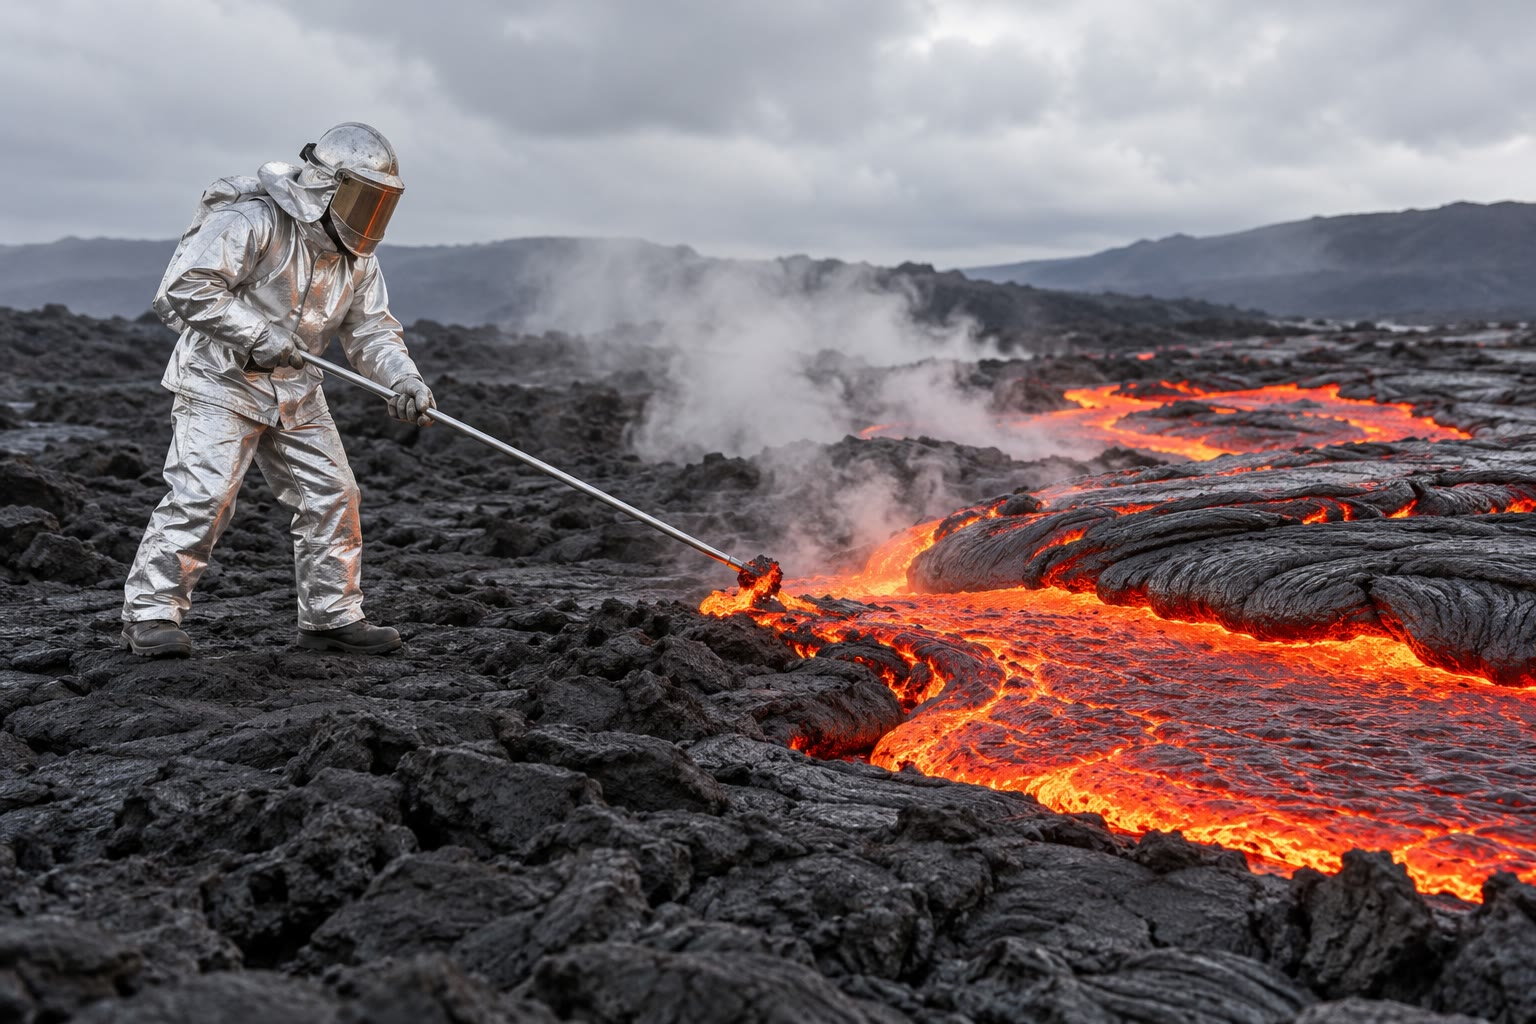
\includegraphics[width=0.6\linewidth]{images/book1/ai/g7-volcanologist.jpg}

{\small Een vulkanoloog in een hittewerend pak neemt met een lange stalen
stok een monster \omterm{def:g4:volcanoes-earthquakes-first-look:eruption}{lava} (door AI gegenereerde illustratie van een algemene
scène). Alleen opgeleide wetenschappers, met dit soort uitrusting, gaan
dicht bij stromende \omterm{def:g4:volcanoes-earthquakes-first-look:eruption}{lava}; alle anderen kijken toe vanaf de plekken die de
autoriteiten toestaan.}
\label{fig:g7:volcanoes:volcanologist}
\end{omfigure}

\section{Twee manieren van uitbarsten}

Mount St.~Helens blies zichzelf op. De \omterm{def:g4:volcanoes-earthquakes-first-look:volcano}{vulkanen} van Hawaï daarentegen
storten meestal \omterm{def:g4:volcanoes-earthquakes-first-look:eruption}{lava} uit die langs hun hellingen wegstroomt. Geologen delen
\omterm{def:g4:volcanoes-earthquakes-first-look:eruption}{uitbarstingen} in twee soorten in.

\begin{definition}[Effusieve en explosieve uitbarstingen]\label{def:g7:volcanoes:eruption-types}
Bij een \emph{effusieve uitbarsting}\index{effusieve uitbarsting} komt het
\omterm{def:g7:volcanoes:magma}{magma} rustig naar buiten als \omterm{def:g4:volcanoes-earthquakes-first-look:eruption}{lava}, die van de \omterm{def:g7:volcanoes:vent}{eruptieopening} wegstroomt,
soms kilometers ver, of in fonteinen van gloeiende druppels omhoogspuit.
Bij een \emph{explosieve uitbarsting}\index{explosieve uitbarsting} wordt
het \omterm{def:g7:volcanoes:magma}{magma} door zijn eigen gas aan stukken geblazen: een kolom van as, gas
en brokken \omterm{def:g3:stones-pebbles-sand:rock}{gesteente} wordt hoog de lucht in geslingerd.
\end{definition}

\begin{omfigure}
\begin{minipage}[t]{0.49\linewidth}\centering
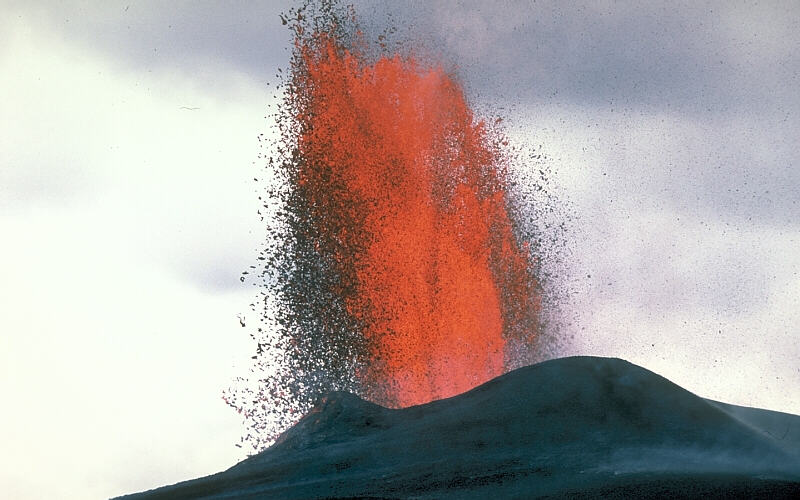
\includegraphics[height=4.5cm]{images/book1/g7-lava-fountain.jpg}

{\small Effusief: een lavafontein op de Kilauea, Hawaï, 1983.
Foto: J.~D. Griggs, USGS.}
\end{minipage}\hfill
\begin{minipage}[t]{0.49\linewidth}\centering
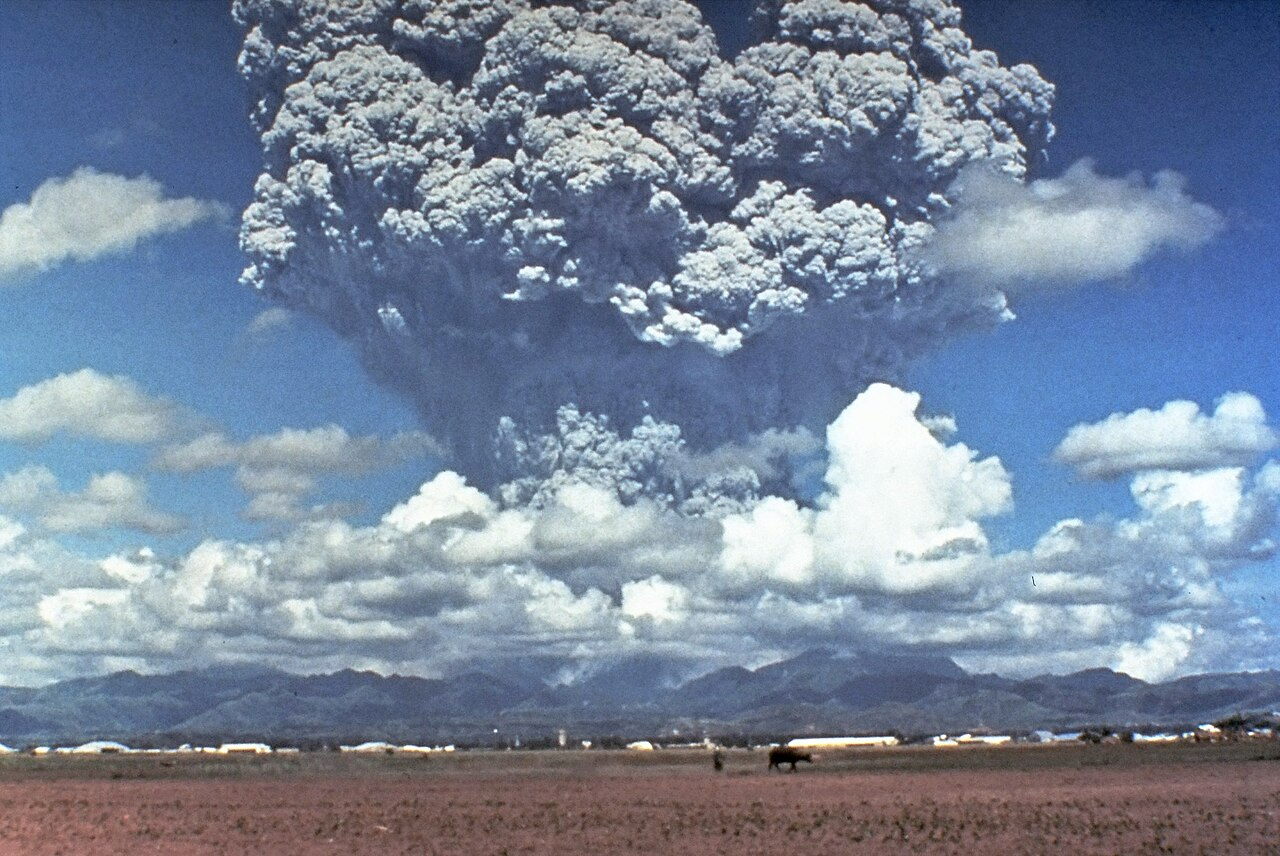
\includegraphics[height=4.5cm]{images/book1/g7-pinatubo.jpg}

{\small Explosief: de eruptiekolom van de Pinatubo, Filipijnen,
12~juni 1991. Foto: Dave Harlow, USGS.}
\end{minipage}\par\medskip


{\small Beide foto's zijn publiek domein (via Wikimedia Commons).}
% ledger: commons:lava-fountain, commons:pinatubo
\label{fig:g7:volcanoes:two-photos}
\end{omfigure}

Wat maakt het verschil? Twee dingen: hoe vloeibaar het \omterm{def:g7:volcanoes:magma}{magma} is, en hoeveel
gas het bevat.

\textbf{Vloeibaar of stroperig.} Sommig \omterm{def:g7:volcanoes:magma}{magma} is vloeibaar, bijna als warme
honing: zo is het \omterm{def:g7:volcanoes:magma}{magma} dat afkoelt tot donker basalt, zoals op Hawaï.
Ander \omterm{def:g7:volcanoes:magma}{magma} is dik en stroperig, als koude honing of tandpasta. Door
vloeibaar \omterm{def:g7:volcanoes:magma}{magma} stijgen gasbellen gemakkelijk op en ontsnappen ze aan het
oppervlak, een paar tegelijk. In stroperig \omterm{def:g7:volcanoes:magma}{magma} zitten de bellen gevangen.

\textbf{Weinig of veel gas.} Een fles bruisend water bevat veel gas dat in
het water is opgelost en daar wordt vastgehouden door de druk in de gesloten
fles; je ziet het niet. Open de fles en de druk daalt: overal verschijnen
bellen, en als de fles geschud is, spuit het schuim eruit. \omterm{def:g7:volcanoes:magma}{Magma} diep onder
de grond bevat ook gas dat onder hoge druk is opgelost. Terwijl het
opstijgt, daalt de druk en komt het gas als bellen uit de oplossing vrij.
% ledger: usgs:volcanic-gases

Zet de twee samen. Vloeibaar \omterm{def:g7:volcanoes:magma}{magma} met weinig gas laat zijn bellen gaan en
komt naar buiten als stromende \omterm{def:g4:volcanoes-earthquakes-first-look:eruption}{lava}: de \omterm{def:g4:volcanoes-earthquakes-first-look:eruption}{uitbarsting} is effusief. Stroperig
\omterm{def:g7:volcanoes:magma}{magma} vol gas houdt zijn bellen vast tot ze zo sterk opzwellen dat ze het
\omterm{def:g7:volcanoes:magma}{magma} aan flarden scheuren: de \omterm{def:g4:volcanoes-earthquakes-first-look:eruption}{uitbarsting} is explosief. De flarden
schuimend \omterm{def:g7:volcanoes:magma}{magma} stollen in de lucht tot as en tot puimsteen, een \omterm{def:g3:stones-pebbles-sand:rock}{gesteente}
zo vol bellen dat het kan drijven.

\begin{example}[Pinatubo, 1991: de verschaalde frisdrank en de geschudde fles]\label{ex:g7:volcanoes:pinatubo}
% ledger: usgs:pinatubo-1991
In juni~1991 bereikte het eerste \omterm{def:g7:volcanoes:magma}{magma} het oppervlak van de Pinatubo, in de
Filipijnen. Op weg naar boven had het het grootste deel van zijn gas
verloren, ``als een fles frisdrank die verschaald is'', in de woorden van de
wetenschappers die de \omterm{def:g4:volcanoes-earthquakes-first-look:volcano}{vulkaan} in de gaten hielden. Het sijpelde langzaam
naar buiten en hoopte zich op tot een \omterm{def:g1:landscapes-around-us:landform}{heuvel} boven de \omterm{def:g7:volcanoes:vent}{eruptieopening}: geen
explosie. Toen, op 12~juni, bereikte \omterm{def:g7:volcanoes:magma}{magma} dat nog vol gas zat het
oppervlak en explodeerde het --- de kolom op de foto hierboven. Op 15~juni
kwam er nog gasrijker \omterm{def:g7:volcanoes:magma}{magma} aan, en had de \omterm{def:g4:volcanoes-earthquakes-first-look:volcano}{vulkaan} een van de grootste
\omterm{def:g4:volcanoes-earthquakes-first-look:eruption}{uitbarstingen} van de twintigste eeuw: hij stootte meer dan vijf kubieke
kilometer \omterm{def:g3:stones-pebbles-sand:rock}{gesteente} en as uit, zijn aswolk steeg tot \qty{35}{km} hoogte,
en de top van de \omterm{def:g1:landscapes-around-us:landform}{berg} stortte in tot een holte van \qty{2.5}{km} doorsnee.
Dezelfde \omterm{def:g4:volcanoes-earthquakes-first-look:volcano}{vulkaan}, dezelfde week: het gas maakte het verschil.
\end{example}

De vorm van een \omterm{def:g4:volcanoes-earthquakes-first-look:volcano}{vulkaan} bewaart de herinnering aan zijn \omterm{def:g4:volcanoes-earthquakes-first-look:eruption}{uitbarstingen}.
Vloeibare \omterm{def:g4:volcanoes-earthquakes-first-look:eruption}{lava} stroomt ver voordat ze hard wordt, dus laag na laag bouwt ze
een brede \omterm{def:g1:landscapes-around-us:landform}{berg} op met flauwe hellingen, met de vorm van een krijgersschild
dat op de grond ligt: een \emph{schildvulkaan}. De Mauna Loa, op Hawaï, is
er een. Stroperige \omterm{def:g4:volcanoes-earthquakes-first-look:eruption}{lava} en as stapelen zich dicht bij de \omterm{def:g7:volcanoes:vent}{eruptieopening} op
tot een steile kegel van lagen \omterm{def:g4:volcanoes-earthquakes-first-look:eruption}{lava} en as: een \emph{stratovulkaan}
(\emph{strata} betekent lagen). Mount St.~Helens en de Pinatubo zijn er
twee.

\begin{omfigure}
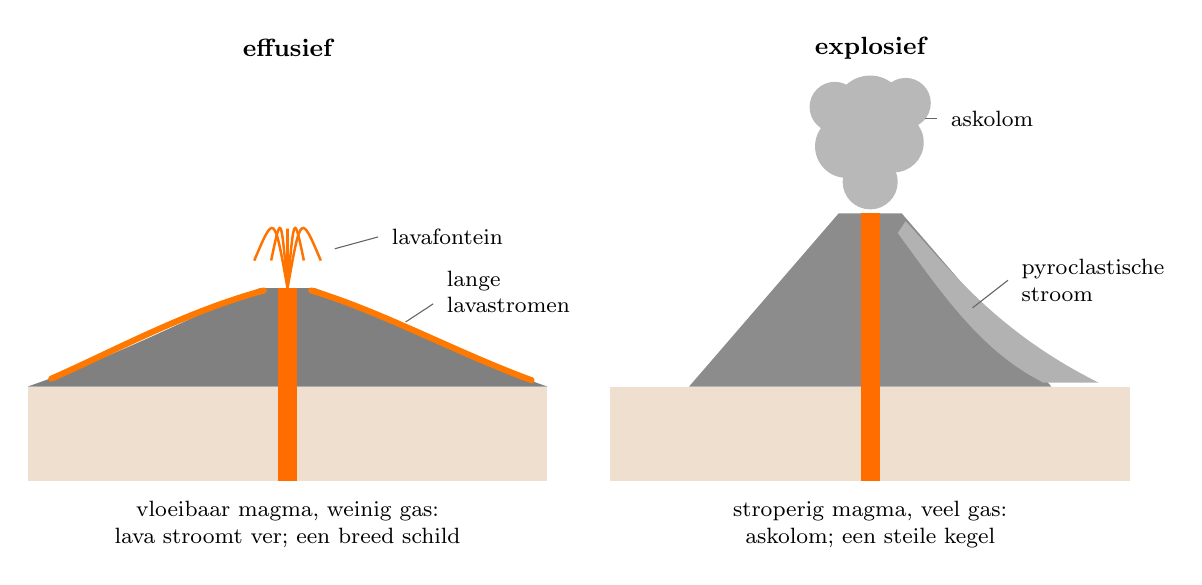
\begin{tikzpicture}[font=\small, x=1cm, y=1cm]
  % --- left: effusive, a shield
  \begin{scope}
    \fill[brown!25] (-3.3,-1.2) rectangle (3.3,0);
    \fill[black!50] (-3.3,0) .. controls (-2.0,0.45) and (-1.0,1.0) .. (-0.35,1.25)
      -- (0.35,1.25) .. controls (1.0,1.0) and (2.0,0.45) .. (3.3,0) -- cycle;
    \fill[orange!85!red] (-0.12,-1.2) rectangle (0.12,1.25);
    % fountain
    \foreach \a in {-25,-12,0,12,25}
      \draw[orange!90!red, line width=0.9pt] (0,1.25) .. controls ({0.4*sin(\a)},2.2) .. ({1.0*sin(\a)},1.6);
    % lava flows far down the gentle slopes
    \draw[orange!95!red, line width=2.2pt, line cap=round] (0.3,1.22) .. controls (1.2,0.95) and (2.1,0.45) .. (3.1,0.08);
    \draw[orange!95!red, line width=2.2pt, line cap=round] (-0.3,1.22) .. controls (-1.3,0.95) and (-2.2,0.45) .. (-3.0,0.1);
    \node[font=\small\bfseries] at (0,4.3) {effusief};
    \node[align=center, font=\footnotesize] at (0,-1.75) {vloeibaar magma, weinig gas:\\lava stroomt ver; een breed schild};
    \node[anchor=west, font=\footnotesize] at (1.2,1.9) {lavafontein};
    \draw[black!60] (1.15,1.9) -- (0.6,1.75);
    \node[anchor=west, font=\footnotesize, align=left] at (1.9,1.2) {lange\\lavastromen};
    \draw[black!60] (1.85,1.05) -- (1.5,0.82);
  \end{scope}
  % --- right: explosive, a steep cone
  \begin{scope}[xshift=7.4cm]
    \fill[brown!25] (-3.3,-1.2) rectangle (3.3,0);
    \fill[black!45] (-2.3,0) -- (-0.4,2.2) -- (0.4,2.2) -- (2.3,0) -- cycle;
    \fill[orange!85!red] (-0.12,-1.2) rectangle (0.12,2.2);
    \foreach \x/\y/\r in {0/2.6/0.35, -0.3/3.05/0.4, 0.3/3.1/0.38, 0/3.5/0.45, -0.45/3.55/0.32, 0.45/3.6/0.32}
      \fill[black!28] (\x,\y) circle (\r);
    % pyroclastic flow down the flank
    \fill[black!30] (0.45,2.1) .. controls (1.0,1.5) and (1.6,0.7) .. (2.9,0.05)
      -- (2.2,0.05) .. controls (1.4,0.45) and (0.9,1.2) .. (0.35,1.95) -- cycle;
    \node[font=\small\bfseries] at (0,4.3) {explosief};
    \node[align=center, font=\footnotesize] at (0,-1.75) {stroperig magma, veel gas:\\askolom; een steile kegel};
    \node[anchor=west, font=\footnotesize] at (0.9,3.4) {askolom};
    \draw[black!60] (0.85,3.4) -- (0.7,3.4);
    \node[anchor=west, font=\footnotesize, align=left] at (1.8,1.35) {pyroclastische\\stroom};
    \draw[black!60] (1.75,1.35) -- (1.3,1.0);
  \end{scope}
\end{tikzpicture}

{\small De twee soorten \omterm{def:g4:volcanoes-earthquakes-first-look:eruption}{uitbarstingen} en de \omterm{def:g4:volcanoes-earthquakes-first-look:volcano}{vulkanen} die ze opbouwen
(tekeningen, niet op schaal).}
\label{fig:g7:volcanoes:two-kinds}
\end{omfigure}

\begin{method}[Effusief of explosief? Vier aanwijzingen]\label{met:g7:volcanoes:clues}
Zoek naar deze aanwijzingen om uit een beschrijving of een foto af te leiden
wat voor \omterm{def:g4:volcanoes-earthquakes-first-look:eruption}{uitbarsting} een \omterm{def:g4:volcanoes-earthquakes-first-look:volcano}{vulkaan} heeft.
\begin{enumerate}
  \item \emph{Wat komt er naar buiten?} \omterm{def:g4:volcanoes-earthquakes-first-look:eruption}{Lava} die stroomt of in fonteinen
        omhoogspuit: effusief. Een askolom, weggeslingerde brokken \omterm{def:g3:stones-pebbles-sand:rock}{gesteente}:
        explosief.
  \item \emph{De vorm van de \omterm{def:g4:volcanoes-earthquakes-first-look:volcano}{vulkaan}.} Een brede \omterm{def:g1:landscapes-around-us:landform}{berg} met flauwe hellingen:
        vooral \omterm{def:g7:volcanoes:eruption-types}{effusieve uitbarstingen}. Een steile kegel: vaak explosief.
  \item \emph{Het \omterm{def:g7:volcanoes:magma}{magma}.} Vloeibaar, weinig gas: effusief. Stroperig, veel
        gas: explosief.
  \item \emph{De \omterm{def:g3:stones-pebbles-sand:rock}{gesteenten} die achterblijven.} Donkere, massieve
        lavastromen: effusief. Lagen as en puimsteen: explosief.
\end{enumerate}
\end{method}

\begin{example}[De aanwijzingen gebruiken]\label{ex:g7:volcanoes:clues}
Een reiziger beschrijft een \omterm{def:g4:volcanoes-earthquakes-first-look:volcano}{vulkaan}: ``een enorme, zacht afgeronde \omterm{def:g1:landscapes-around-us:landform}{berg},
overal zwarte lavastromen op de hellingen, sommige pas een paar jaar
oud''. Aanwijzing~2 (flauwe hellingen) en aanwijzing~4 (donkere
lavastromen) wijzen allebei op \omterm{def:g7:volcanoes:eruption-types}{effusieve uitbarstingen}: het is een
schildvulkaan, zoals de Mauna Loa.
\end{example}

\begin{inthelab}[Een vulkaan in een fles (in de klas, met de leraar)]
De leraar neemt twee gesloten flessen bruisend water. De ene heeft stil
gestaan; de andere is zachtjes geschud. Beide worden buiten geopend, boven
een teil, weggericht van iedereen. De stille fles sist en laat een paar
bellen opstijgen; de geschudde barst uit in schuim dat eruit spuit. Welke
fles lijkt op het \omterm{def:g7:volcanoes:magma}{magma} van Hawaï, welke op dat van de Pinatubo? Laat
daarna een stukje puimsteen en een \omterm{def:g3:stones-pebbles-sand:pebble}{kiezel} in een kom water vallen: de
puimsteen drijft. Bekijk hem door een vergrootglas: hij zit vol gaatjes, de
gasbellen die in het \omterm{def:g3:stones-pebbles-sand:rock}{gesteente} zijn gestold toen het \omterm{def:g7:volcanoes:magma}{magma} uiteenspatte.
\end{inthelab}

\section{Wat er uit een vulkaan komt}

Een \omterm{def:g4:volcanoes-earthquakes-first-look:eruption}{uitbarsting} stoot veel meer uit dan \omterm{def:g4:volcanoes-earthquakes-first-look:eruption}{lava}: gassen, as, brokken \omterm{def:g3:stones-pebbles-sand:rock}{gesteente}
en, in de ergste gevallen, lawines van hete as.

Verreweg het meest voorkomende gas is waterdamp. Grote \omterm{def:g4:volcanoes-earthquakes-first-look:eruption}{uitbarstingen} stoten
in korte tijd enorme hoeveelheden gas uit: op één enkele dag in 1991 zou de
Pinatubo meer dan 250~miljoen ton gas de hogere atmosfeer in hebben
gestuurd.
% ledger: usgs:volcanic-gases

\begin{definition}[Pyroclastische stroom]\label{def:g7:volcanoes:pyroclastic-flow}
Een \emph{pyroclastische stroom}\index{pyroclastische stroom} is een snelle
lawine van heet gas, as en stukken \omterm{def:g3:stones-pebbles-sand:rock}{gesteente}, van stofkorrels tot
rotsblokken, die tijdens een \omterm{def:g7:volcanoes:eruption-types}{explosieve uitbarsting} langs de hellingen van
een \omterm{def:g4:volcanoes-earthquakes-first-look:volcano}{vulkaan} omlaag raast. (\emph{Pyro} betekent vuur en \emph{klastisch}
betekent opgebouwd uit gebroken stukken.)
\end{definition}

Pyroclastische stromen bewegen meestal sneller dan \qty{80}{km/h}, en het
\omterm{def:g3:stones-pebbles-sand:rock}{gesteente} en gas erin zijn doorgaans tussen 200 en
\qty{700}{\degreeCelsius} heet. Ze volgen meestal de \omterm{def:g1:landscapes-around-us:landform}{dalen}, net als water,
en slaan bijna alles op hun pad omver, verbranden het of begraven het. Op
18~mei 1980 raasden de pyroclastische stromen van Mount St.~Helens met 80
tot \qty{130}{km/h} omlaag, bij een temperatuur van minstens
\qty{700}{\degreeCelsius}, en kwamen ze tot \qty{8}{km} van de \omterm{def:g7:volcanoes:vent}{krater}.
% ledger: usgs:pyroclastic-flows, usgs:msh-flows, usgs:msh-reach

De tabel vat de producten van een \omterm{def:g4:volcanoes-earthquakes-first-look:volcano}{vulkaan} samen.

\begin{center}
\small
\begin{tabular}{|p{0.2\linewidth}|p{0.4\linewidth}|p{0.3\linewidth}|}
\hline
\textbf{product} & \textbf{wat het is} & \textbf{het gevaar} \\
\hline
lavastroom & gesmolten \omterm{def:g3:stones-pebbles-sand:rock}{gesteente} dat over de grond stroomt en daarna hard wordt & verbrandt en begraaft wat het tegenkomt, maar is meestal traag genoeg om mensen uit de weg te laten gaan \\
\hline
as & piepkleine stukjes \omterm{def:g3:stones-pebbles-sand:rock}{gesteente} en glas, de lucht in geblazen & valt ver weg neer; daken bezwijken onder het gewicht; beschadigt vliegtuigen \\
\hline
vulkanische bommen & weggeslingerde klonten \omterm{def:g4:volcanoes-earthquakes-first-look:eruption}{lava} die tijdens hun vlucht hard worden & verpletteren wat ze raken, dicht bij de \omterm{def:g7:volcanoes:vent}{eruptieopening} \\
\hline
gassen & vooral waterdamp, daarna koolstofdioxide en zwaveldioxide & sommige zijn giftig; koolstofdioxide verzamelt zich in laagten \\
\hline
\omterm{def:g7:volcanoes:pyroclastic-flow}{pyroclastische stroom} & een lawine van hete as, \omterm{def:g3:stones-pebbles-sand:rock}{gesteente} en gas & de dodelijkste: te snel en te heet om eraan te ontkomen \\
\hline
modderstroom & as en \omterm{def:g3:stones-pebbles-sand:rock}{gesteente} vermengd met water van \omterm{def:g4:clouds-rain-snow:precipitation}{regen} of gesmolten \omterm{def:g4:clouds-rain-snow:precipitation}{sneeuw} & raast door \omterm{def:g1:landscapes-around-us:landform}{dalen} omlaag, soms ver van de \omterm{def:g4:volcanoes-earthquakes-first-look:volcano}{vulkaan} \\
\hline
\end{tabular}
\end{center}
% ledger: usgs:lava-flows, usgs:volcanic-gases, usgs:pyroclastic-flows, usgs:pinatubo-1991, usgs:msh-flows

\begin{method}[Hoe lang duurt het?]\label{met:g7:volcanoes:time}
Om te vinden hoe lang iets dat met een bekende snelheid beweegt erover doet
om een afstand af te leggen, deel je de afstand door de snelheid:
\[
\text{tijd} = \frac{\text{afstand}}{\text{snelheid}}.
\]
Met een afstand in kilometer en een snelheid in kilometer per uur komt de
tijd uit in uren; vermenigvuldig met 60 om minuten te krijgen.
\end{method}

\begin{example}[Een race tegen een pyroclastische stroom]\label{ex:g7:volcanoes:race}
Een \omterm{def:g7:volcanoes:pyroclastic-flow}{pyroclastische stroom} die met \qty{120}{km/h} beweegt, gaat af op een
dorp \qty{6}{km} verderop in het \omterm{def:g1:landscapes-around-us:landform}{dal}. Hij doet er $6 \div 120 = 0.05$~uur
over, dat is $0.05 \times 60 = 3$~minuten. Drie minuten: niemand kan op tijd
het \omterm{def:g1:landscapes-around-us:landform}{dal} uit rennen, of zelfs rijden. Mensen zijn alleen veilig als ze
\emph{voor} de \omterm{def:g4:volcanoes-earthquakes-first-look:eruption}{uitbarsting} zijn vertrokken.
\end{example}

\begin{remark}[Modderstromen: het gevaar dat later komt]\label{rem:g7:volcanoes:mudflows}
% ledger: usgs:msh-flows, usgs:pinatubo-lahars
Een \omterm{def:g4:volcanoes-earthquakes-first-look:eruption}{uitbarsting} laat de hellingen bedekt met losse as achter. Als er \omterm{def:g4:clouds-rain-snow:precipitation}{regen}
op valt, of als de hitte de \omterm{def:g4:clouds-rain-snow:precipitation}{sneeuw} en het ijs van de top doet smelten,
verandert de as in modderstromen die door de \omterm{def:g1:landscapes-around-us:landform}{dalen} omlaag razen. Op
18~mei 1980 beschadigden de modderstromen van Mount St.~Helens 27~bruggen
en bijna 200~woningen. Rond de Pinatubo veranderden de zware \omterm{def:g4:clouds-rain-snow:precipitation}{regens} van de
jaren daarna de as in reusachtige modderstromen die hele dorpen begroeven:
ze richtten meer schade aan dan de \omterm{def:g4:volcanoes-earthquakes-first-look:eruption}{uitbarsting} zelf.
\end{remark}


\section{Waar liggen de vulkanen?}

De Smithsonian Institution in Washington houdt een lijst bij van alle
\omterm{def:g4:volcanoes-earthquakes-first-look:volcano}{vulkanen} waarvan bekend is dat ze in de laatste 12\,000 jaar zijn
uitgebarsten: 1\,214 in totaal, op het land en onder de \omterm{def:g2:water-on-earth:ocean}{zee}. Voor elke
\omterm{def:g4:volcanoes-earthquakes-first-look:volcano}{vulkaan} vermeldt de lijst waar hij ligt ten opzichte van de \omterm{def:g7:plate-tectonics:plate}{platen}. De \omterm{def:g2:drawing-to-map:map}{kaart}
hieronder kleurt ze op die manier.
% ledger: data:gvp (counts computed in figdata/grade-7/volcano_settings.py)

\begin{omfigure}
\begin{tikzpicture}
\begin{axis}[ommap, width=\linewidth, xtick={-180,-90,...,180}, ytick={-60,0,60},
  legend style={at={(0.02,0.04)}, anchor=south west, font=\scriptsize,
  fill=white, fill opacity=0.85, text opacity=1, draw=black!40}, legend cell align=left]
\addplot[fill=omLithAlluv, draw=black!45, line width=0.2pt, forget plot] table {figdata/out/shared-geo-land.dat};
\addplot[omRidge!60, line width=0.5pt, forget plot] table {figdata/out/shared-geo-school-ridge.dat};
\addplot[omTrench!60, line width=0.5pt, forget plot] table {figdata/out/shared-geo-school-subduction.dat};
\addplot[only marks, mark=triangle*, mark size=1.3pt, omTrench, forget plot] table {figdata/out/grade-7-volcano_settings-map-sub.dat};
\addplot[only marks, mark=triangle*, mark size=1.3pt, omRidge, forget plot] table {figdata/out/grade-7-volcano_settings-map-rift.dat};
\addplot[only marks, mark=*, mark size=1.4pt, orange!90!black, forget plot] table {figdata/out/grade-7-volcano_settings-map-intra.dat};
\addlegendimage{only marks, mark=triangle*, mark size=1.6pt, omTrench}
\addlegendentry{waar een plaat onder een andere zakt}
\addlegendimage{only marks, mark=triangle*, mark size=1.6pt, omRidge}
\addlegendentry{waar platen uit elkaar bewegen}
\addlegendimage{only marks, mark=*, mark size=1.6pt, orange!90!black}
\addlegendentry{binnen een plaat}
\end{axis}
\end{tikzpicture}

{\small De \omterm{def:g4:volcanoes-earthquakes-first-look:volcano}{vulkanen} die in de laatste 12\,000 jaar actief waren, gekleurd
naar hun ligging. Vage lijnen: de \omterm{def:g7:plate-tectonics:plate-boundary}{plaatgrenzen} waar \omterm{def:g7:plate-tectonics:plate}{platen} uit elkaar
bewegen (rood) en waar een \omterm{def:g7:plate-tectonics:plate}{plaat} onder een andere zakt (blauw). Gegevens:
Smithsonian Global Volcanism Program; \omterm{def:g7:plate-tectonics:plate-boundary}{plaatgrenzen} naar P.~Bird (2003);
kustlijnen van Natural Earth.}
% ledger: data:gvp, data:pb2002, data:ne-land
\label{fig:g7:volcanoes:map}
\end{omfigure}

\begin{omfigure}
\begin{tikzpicture}
  \begin{axis}[xbar, width=0.72\linewidth, height=3.6cm, bar width=8pt,
      xmin=0, xmax=1000, ymin=-0.6, ymax=3.6, y dir=reverse,
      ytick={0,...,3}, yticklabels={{waar een plaat onder een andere zakt},{waar platen uit elkaar bewegen},{binnen een plaat},{onbekend}},
      xlabel={aantal vulkanen},
      axis x line=bottom, axis y line=left, axis line style={-},
      tick label style={font=\scriptsize}, label style={font=\small},
      nodes near coords, nodes near coords style={font=\scriptsize, anchor=west},
      point meta=explicit symbolic, enlarge y limits=false, clip=false]
    \addplot[fill=black!30, draw=black!60] table[x=n, y=idx, meta=n] {figdata/out/grade-7-volcano_settings.dat};
  \end{axis}
\end{tikzpicture}

{\small Hoeveel van de 1\,214 \omterm{def:g4:volcanoes-earthquakes-first-look:volcano}{vulkanen} in elke ligging staan.}
% ledger: data:gvp (figdata/grade-7/volcano_settings.py, main table)
\label{fig:g7:volcanoes:counts}
\end{omfigure}

\begin{proposition}[De meeste vulkanen staan op plaatgrenzen]\label{prop:g7:volcanoes:where}
% ledger: data:gvp (counts computed in figdata/grade-7/volcano_settings.py)
Van de 1\,214 \omterm{def:g4:volcanoes-earthquakes-first-look:volcano}{vulkanen} die in de laatste 12\,000 jaar actief waren, staan er
838 (69~\%) waar een \omterm{def:g7:plate-tectonics:plate}{plaat} onder een andere zakt en 221 (18~\%) waar \omterm{def:g7:plate-tectonics:plate}{platen}
uit elkaar bewegen; 149 (12~\%) staan binnen een \omterm{def:g7:plate-tectonics:plate}{plaat}, ver van de randen.
Van de laatste 6 (0.5~\%) is de ligging onbekend.
\end{proposition}

\textbf{Waar \omterm{def:g7:plate-tectonics:plate}{platen} uit elkaar bewegen.} Langs de oceanische ruggen, en in
slenken zoals die welke Oost-Afrika uiteenscheurt, trekken de \omterm{def:g7:plate-tectonics:plate}{platen} van
elkaar weg. \omterm{def:g7:volcanoes:magma}{Magma} stijgt uit de \omterm{def:g6:inside-the-earth:layers}{mantel} op in de wijder wordende spleten en
vult ze: er wordt nieuwe \omterm{def:g6:inside-the-earth:layers}{aardkorst} gemaakt. De meeste ruggen liggen onder
de \omterm{def:g2:water-on-earth:ocean}{zee}, maar IJsland ligt precies op de Midden-Atlantische Rug: daar zijn
deze \omterm{def:g4:volcanoes-earthquakes-first-look:volcano}{vulkanen} op het land te zien. Hun \omterm{def:g7:volcanoes:magma}{magma} is meestal vloeibaar basalt,
en hun \omterm{def:g4:volcanoes-earthquakes-first-look:eruption}{uitbarstingen} zijn meestal effusief.
% ledger: usgs:arc-magma, usgs:iceland, usgs:east-africa

\textbf{Waar een \omterm{def:g7:plate-tectonics:plate}{plaat} onder een andere zakt.} Meer dan twee op de drie
\omterm{def:g4:volcanoes-earthquakes-first-look:volcano}{vulkanen} staan hier, langs lijnen die de randen van de Stille \omterm{def:g2:water-on-earth:ocean}{Oceaan} volgen
--- de ``Ring van Vuur'' --- en op een paar andere plaatsen. Diep onder de
grond, langs de zakkende \omterm{def:g7:plate-tectonics:plate}{plaat}, smelt een deel van het \omterm{def:g3:stones-pebbles-sand:rock}{gesteente}
gedeeltelijk; wetenschappers discussiëren nog over welk \omterm{def:g3:stones-pebbles-sand:rock}{gesteente} precies
smelt, de zakkende \omterm{def:g7:plate-tectonics:plate}{plaat} of de \omterm{def:g7:plate-tectonics:plate}{plaat} erboven, of allebei. Het \omterm{def:g7:volcanoes:magma}{magma} dat
daar opstijgt, is vaak stroperig en vol gas: dit zijn de explosieve
\omterm{def:g4:volcanoes-earthquakes-first-look:volcano}{vulkanen}, zoals Mount St.~Helens en de Pinatubo. De gegevens laten het
zien: van de 660 steile kegels (stratovulkanen) in de lijst staan er 564
--- dat is 85~\% --- waar een \omterm{def:g7:plate-tectonics:plate}{plaat} onder een andere zakt.
% ledger: usgs:arc-magma, data:gvp (figdata/grade-7/volcano_settings.py, part strato)

\textbf{Binnen een \omterm{def:g7:plate-tectonics:plate}{plaat}.} Een paar \omterm{def:g4:volcanoes-earthquakes-first-look:volcano}{vulkanen} liggen ver van elke
\omterm{def:g7:plate-tectonics:plate-boundary}{plaatgrens}. De bekendste zijn die van Hawaï, midden in de Stille \omterm{def:g2:water-on-earth:ocean}{Oceaan},
meer dan \qty{3200}{km} van de dichtstbijzijnde plaatrand.
% ledger: usgs:hawaii-hotspot

\begin{definition}[Hotspot]\label{def:g7:volcanoes:hotspot}
Een \emph{hotspot}\index{hotspot} is een plek diep in de \omterm{def:g6:inside-the-earth:layers}{mantel} die
miljoenen jaren heet blijft en \omterm{def:g4:volcanoes-earthquakes-first-look:volcano}{vulkanen} aan het oppervlak van \omterm{def:g7:volcanoes:magma}{magma} blijft
voorzien, zelfs ver van de randen van de \omterm{def:g7:plate-tectonics:plate}{platen}.
\end{definition}

De \omterm{def:g7:volcanoes:hotspot}{hotspot} blijft waar hij is, terwijl de \omterm{def:g7:plate-tectonics:plate}{plaat} erboven beweegt. Boven de
\omterm{def:g7:volcanoes:hotspot}{hotspot} groeit een \omterm{def:g4:volcanoes-earthquakes-first-look:volcano}{vulkaan}; daarna voert de bewegende \omterm{def:g7:plate-tectonics:plate}{plaat} hem mee en
dooft hij uit, terwijl achter hem een nieuwe \omterm{def:g4:volcanoes-earthquakes-first-look:volcano}{vulkaan} boven de \omterm{def:g7:volcanoes:hotspot}{hotspot}
groeit. Na verloop van tijd draagt de \omterm{def:g7:plate-tectonics:plate}{plaat} een hele rij \omterm{def:g4:volcanoes-earthquakes-first-look:volcano}{vulkanen}, met de
oudste het verst van de \omterm{def:g7:volcanoes:hotspot}{hotspot}. Dat is precies wat we op Hawaï zien: de
oudste \omterm{def:g3:stones-pebbles-sand:rock}{gesteenten} van het eiland Kauai, aan het noordwestelijke uiteinde
van de bewoonde eilanden, zijn ongeveer 5.5~miljoen jaar oud en diep
uitgesleten door \omterm{def:g4:clouds-rain-snow:precipitation}{regen} en golven; op Big Island, aan het zuidoostelijke
uiteinde, zijn de oudste \omterm{def:g3:stones-pebbles-sand:rock}{gesteenten} aan het oppervlak minder dan
0.7~miljoen jaar oud, en komt er nog steeds nieuwe \omterm{def:g4:volcanoes-earthquakes-first-look:eruption}{lava} naar buiten.
% ledger: usgs:hawaii-hotspot

\begin{history}[Een geofysicus en een rij eilanden]
% ledger: usgs:hawaii-hotspot
Waarom zou er midden in de grootste \omterm{def:g7:plate-tectonics:plate}{plaat} op Aarde een keten van
vulkanische eilanden oprijzen? In 1963 stelde de Canadese geofysicus
J.~Tuzo Wilson een antwoord voor. De Hawaïaanse eilanden, opperde hij,
liggen op een rij omdat de Pacifische \omterm{def:g7:plate-tectonics:plate}{plaat} beweegt over een diepe, vaste
warmtebron in de \omterm{def:g6:inside-the-earth:layers}{mantel}, die de \omterm{def:g7:plate-tectonics:plate}{plaat} erboven gedeeltelijk doet smelten.
Als hij gelijk had, moesten de eilanden ouder en meer uitgesleten zijn
naarmate ze verder van de actieve \omterm{def:g4:volcanoes-earthquakes-first-look:volcano}{vulkanen} van Big Island liggen. De
ouderdom van hun \omterm{def:g3:stones-pebbles-sand:rock}{gesteenten} laat precies dat zien. Eén enkel idee verklaarde
zowel de rij als de volgorde van de ouderdommen. (Wilson is ook de
wetenschapper die de transforme grenzen ontdekte, waar \omterm{def:g7:plate-tectonics:plate}{platen} langs elkaar
schuiven.)
\end{history}

\begin{omfigure}
\begin{tikzpicture}[font=\small, x=1cm, y=1cm]
  % sea, plate and mantle
  \fill[omSea!45] (-6.2,0) rectangle (6.2,1.0);
  \fill[orange!12] (-6.2,-3.4) rectangle (6.2,-1.0);
  \fill[brown!35] (-6.2,-1.0) rectangle (6.2,0);
  \draw[omSea!80!black, line width=0.5pt] (-6.2,1.0) -- (6.2,1.0);
  \node[font=\footnotesize] at (-4.6,-0.5) {Pacifische plaat};
  % the hotspot plume, fixed in the mantle, and the magma rising to the volcano
  \fill[orange!80!red] (4.0,-3.4) .. controls (3.6,-2.4) .. (3.75,-1.0) -- (4.25,-1.0) .. controls (4.4,-2.4) .. (4.0,-3.4) -- cycle;
  \node[anchor=west, align=left, font=\footnotesize] at (4.5,-2.5) {hotspot: blijft\\op zijn plaats};
  % volcanoes rise from the sea floor; youngest over the hotspot
  \fill[black!55] (2.3,0) .. controls (3.2,1.2) .. (3.75,1.85) -- (4.25,1.85) .. controls (4.8,1.2) .. (5.7,0) -- cycle;
  \fill[orange!80!red] (3.93,-1.0) rectangle (4.07,1.85);
  \fill[black!45] (-0.4,0) .. controls (0.4,0.9) .. (0.9,1.3) -- (1.3,1.3) .. controls (1.8,0.9) .. (2.6,0) -- cycle;
  \fill[black!35] (-3.2,0) .. controls (-2.5,0.6) .. (-2.1,0.8) -- (-1.7,0.8) .. controls (-1.3,0.6) .. (-0.6,0) -- cycle;
  \fill[black!28] (-5.8,0) .. controls (-5.2,0.4) .. (-4.9,0.5) -- (-4.6,0.5) .. controls (-4.3,0.4) .. (-3.6,0) -- cycle;
  % labels
    \node[align=center, font=\footnotesize, anchor=south] at (4.3,1.95) {actieve vulkaan\\(Big Island: minder\\dan 0.7 miljoen jaar)};
  \node[align=center, font=\footnotesize, anchor=south] at (0.7,1.4) {oud, uitgesleten eiland\\(Kauai: ongeveer\\5.5 miljoen jaar)};
  \node[align=center, font=\footnotesize] at (-1.9,1.5) {oudere vulkaan,\\onder de golven};
  \node[align=center, font=\footnotesize] at (-4.75,1.3) {nog ouder,\\wegzakkend};
  \node[font=\footnotesize] at (5.75,0.55) {zee};
  \node[font=\footnotesize] at (-4.3,-2.2) {mantel};
  % plate motion
  \draw[-{Stealth[length=3mm]}, line width=1.2pt] (2.2,-0.62) -- (-1.8,-0.62);
  \node[font=\footnotesize] at (0.2,-0.28) {de plaat beweegt naar het noordwesten};
    \node[font=\footnotesize\bfseries] at (-5.8,-3.1) {NW};
  \node[font=\footnotesize\bfseries] at (5.8,-3.1) {ZO};
\end{tikzpicture}

{\small Een \omterm{def:g7:plate-tectonics:plate}{plaat} die over een \omterm{def:g7:volcanoes:hotspot}{hotspot} beweegt (een tekening, niet op schaal;
de eilanden ertussen zijn weggelaten). De \omterm{def:g4:volcanoes-earthquakes-first-look:volcano}{vulkaan} boven de \omterm{def:g7:volcanoes:hotspot}{hotspot} is jong
en actief; de \omterm{def:g7:plate-tectonics:plate}{plaat} voert de oudere \omterm{def:g4:volcanoes-earthquakes-first-look:volcano}{vulkanen} mee naar het noordwesten, waar
ze uitdoven, uitslijten en ten slotte onder de golven verdwijnen.}
% ledger: usgs:hawaii-hotspot
\label{fig:g7:volcanoes:hotspot}
\end{omfigure}

\begin{omfigure}
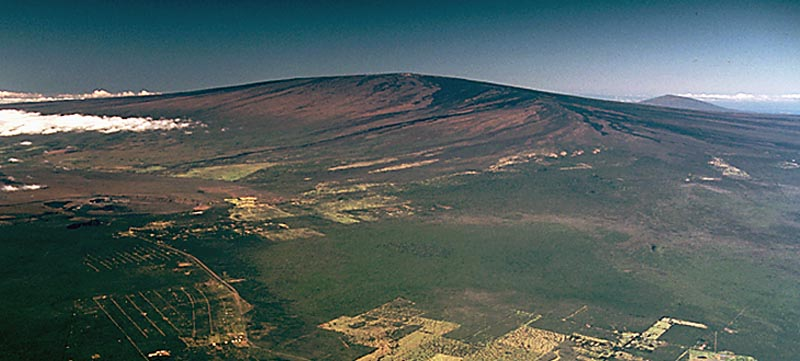
\includegraphics[width=0.8\linewidth]{images/book1/g7-mauna-loa.jpg}

{\small De Mauna Loa, een schildvulkaan op Big Island (Hawaï), gezien vanuit
de lucht: een enorme \omterm{def:g1:landscapes-around-us:landform}{berg} met flauwe hellingen, opgebouwd door duizenden
vloeibare lavastromen. Foto: J.~D. Griggs, U.S. Geological Survey, 1985
(publiek domein, via Wikimedia Commons).}
% ledger: commons:mauna-loa
\label{fig:g7:volcanoes:mauna-loa}
\end{omfigure}

\section{Leven met vulkanen}

Veel mensen wonen in de buurt van \omterm{def:g4:volcanoes-earthquakes-first-look:volcano}{vulkanen}: in 1991 woonden er ongeveer
3~miljoen in de streek rond de Pinatubo. Gelukkig geeft een grote
\omterm{def:g4:volcanoes-earthquakes-first-look:eruption}{uitbarsting} vaak waarschuwingssignalen. Opstijgend \omterm{def:g7:volcanoes:magma}{magma} duwt het \omterm{def:g3:stones-pebbles-sand:rock}{gesteente}
opzij: de grond scheurt en schudt met kleine \omterm{def:g4:volcanoes-earthquakes-first-look:earthquake}{aardbevingen}, de hellingen
zwellen op, er ontsnapt gas. Bij Mount St.~Helens kwamen de eerste kleine
\omterm{def:g4:volcanoes-earthquakes-first-look:earthquake}{aardbevingen} op 16~maart 1980; tegen 17~mei waren het er meer dan 10\,000,
en de noordflank was minstens \qty{137}{m} naar buiten opgezwollen.
Wetenschappers maten dit allemaal en het gebied werd afgesloten; toch
kwamen er op 18~mei 57~mensen om.
% ledger: usgs:msh-lead-up, usgs:msh-flows

Bij de Pinatubo gaven in 1991 de wetenschappers die de \omterm{def:g4:volcanoes-earthquakes-first-look:earthquake}{aardbevingen}, het gas
en het opzwellen van de \omterm{def:g4:volcanoes-earthquakes-first-look:volcano}{vulkaan} volgden op tijd de waarschuwing: de mensen
die bij de \omterm{def:g4:volcanoes-earthquakes-first-look:volcano}{vulkaan} woonden vertrokken, en er werden minstens 5\,000 levens
gered.
% ledger: usgs:pinatubo-1991 (central Luzon home to about 3 million people)

\begin{remark}[Ga nooit naar een vulkaan die uitbarst]\label{rem:g7:volcanoes:safety}
Naar een \omterm{def:g4:volcanoes-earthquakes-first-look:eruption}{uitbarsting} kijken mag alleen op de plekken die de autoriteiten
voor het publiek hebben opengesteld. Gassen, vallende stenen, verse
lavakorst die onder je voeten breekt en pyroclastische stromen kunnen
dodelijk zijn, vaak zonder waarschuwing. Vulkaanobservatoria maken bekend
wat veilig te bezoeken is: volg hun aanwijzingen altijd op.
\end{remark}

\section{Oefeningen}

\begin{exercise}[$\star$]\label{exo:g7:volcanoes:1}
Koppel elk woord aan zijn betekenis: \omterm{def:g7:volcanoes:magma}{magma}; \omterm{def:g4:volcanoes-earthquakes-first-look:eruption}{lava}; \omterm{def:g7:volcanoes:magma-chamber}{magmakamer};
\omterm{def:g7:volcanoes:vent}{eruptieopening}; \omterm{def:g7:volcanoes:vent}{krater}. (a) Een komvormige holte op de top van een \omterm{def:g4:volcanoes-earthquakes-first-look:volcano}{vulkaan}.
(b) Gesmolten \omterm{def:g3:stones-pebbles-sand:rock}{gesteente} onder de grond. (c) Een opening waardoor \omterm{def:g7:volcanoes:magma}{magma} naar
buiten komt. (d) Gesmolten \omterm{def:g3:stones-pebbles-sand:rock}{gesteente} dat aan het oppervlak is gekomen.
(e) Een grote holte vol \omterm{def:g7:volcanoes:magma}{magma} een paar kilometer onder een \omterm{def:g4:volcanoes-earthquakes-first-look:volcano}{vulkaan}.
\end{exercise}

\begin{exercise}[$\star$]\label{exo:g7:volcanoes:2}
Effusief of explosief? (a) \omterm{def:g1:landscapes-around-us:water}{Rivieren} van gloeiende \omterm{def:g4:volcanoes-earthquakes-first-look:eruption}{lava} stromen een flauwe
helling af. (b) Een askolom stijgt \qty{35}{km} de lucht in. (c) Uit een
spleet spuit een fontein van gloeiende druppels. (d) Een lawine van hete
as en gas raast een \omterm{def:g1:landscapes-around-us:landform}{dal} in.
\end{exercise}

\begin{exercise}[$\star$]\label{exo:g7:volcanoes:3}
Waar of niet waar? Verbeter de onware uitspraken. (a) \omterm{def:g7:volcanoes:magma}{Magma} en \omterm{def:g4:volcanoes-earthquakes-first-look:eruption}{lava} zijn
twee namen voor hetzelfde gesmolten \omterm{def:g3:stones-pebbles-sand:rock}{gesteente}, onder de grond en aan het
oppervlak. (b) Het meest voorkomende vulkanische gas is koolstofdioxide.
(c) Een \omterm{def:g7:volcanoes:pyroclastic-flow}{pyroclastische stroom} is een \omterm{def:g1:landscapes-around-us:water}{rivier} van vloeibare \omterm{def:g4:volcanoes-earthquakes-first-look:eruption}{lava}. (d) De
\omterm{def:g4:volcanoes-earthquakes-first-look:volcano}{vulkanen} van Hawaï staan op een \omterm{def:g7:plate-tectonics:plate-boundary}{plaatgrens}.
\end{exercise}

\begin{exercise}[$\star$]\label{exo:g7:volcanoes:4}
Gebruik de tabel van de gloeikleuren. (a) \omterm{def:g4:volcanoes-earthquakes-first-look:eruption}{Lava} gloeit geel: geef de
temperatuur. (b) Een lavastroom die hard wordt, gloeit donkerrood: geef de
temperatuur. (c) Een foto toont oranje \omterm{def:g4:volcanoes-earthquakes-first-look:eruption}{lava} aan het front van een
lavastroom en gele \omterm{def:g4:volcanoes-earthquakes-first-look:eruption}{lava} bij de \omterm{def:g7:volcanoes:vent}{eruptieopening}. Waar is het heter? Waarom?
\end{exercise}

\begin{exercise}[$\star\star$]\label{exo:g7:volcanoes:5}
Gebruik het staafdiagram van de 1\,214 \omterm{def:g4:volcanoes-earthquakes-first-look:volcano}{vulkanen}. (a) Hoeveel \omterm{def:g4:volcanoes-earthquakes-first-look:volcano}{vulkanen} staan
op een \omterm{def:g7:plate-tectonics:plate-boundary}{plaatgrens} (waar \omterm{def:g7:plate-tectonics:plate}{platen} uit elkaar bewegen, of waar de ene onder de
andere zakt)? (b) Welk percentage van alle \omterm{def:g4:volcanoes-earthquakes-first-look:volcano}{vulkanen} is dat? (c) Controleer
dat de drie percentages van de propositie, samen met de 6 \omterm{def:g4:volcanoes-earthquakes-first-look:volcano}{vulkanen} met een
onbekende ligging (0.5~\%), ongeveer 100~\% opleveren.
\end{exercise}

\begin{exercise}[$\star\star$]\label{exo:g7:volcanoes:6}
Van de 660 steile kegels (stratovulkanen) in de lijst staan er 564 waar een
\omterm{def:g7:plate-tectonics:plate}{plaat} onder een andere zakt, 62 waar \omterm{def:g7:plate-tectonics:plate}{platen} uit elkaar bewegen en 33 binnen
een \omterm{def:g7:plate-tectonics:plate}{plaat}. (a) Bereken het percentage steile kegels dat staat waar een \omterm{def:g7:plate-tectonics:plate}{plaat}
onder een andere zakt. (b) Hoeveel steile kegels blijven er over voor de
ligging ``onbekend''? (c) Gebruik de vier aanwijzingen: wat voor
\omterm{def:g4:volcanoes-earthquakes-first-look:eruption}{uitbarstingen} verwachten we langs de Ring van Vuur?
\end{exercise}

\begin{exercise}[$\star\star$]\label{exo:g7:volcanoes:7}
Bij de Kilauea verlaat \omterm{def:g4:volcanoes-earthquakes-first-look:eruption}{lava} de \omterm{def:g7:volcanoes:vent}{eruptieopening} bij ongeveer
\qty{1170}{\degreeCelsius}. In een lavatunnel bereikte ze de \omterm{def:g2:water-on-earth:ocean}{zee},
\qty{10}{km} verderop, bij ongeveer \qty{1140}{\degreeCelsius}. (a) Hoeveel
graden is ze afgekoeld? (b) Hoeveel graden is dat per kilometer? (c) \omterm{def:g4:volcanoes-earthquakes-first-look:eruption}{Lava} in
de open lucht koelt aan het oppervlak honderden graden per seconde af. Leg
uit waarom de \omterm{def:g4:volcanoes-earthquakes-first-look:eruption}{lava} in de tunnel zo heet bleef.
\end{exercise}

\begin{exercise}[$\star\star$]\label{exo:g7:volcanoes:8}
De oudste \omterm{def:g3:stones-pebbles-sand:rock}{gesteenten} van Kauai zijn ongeveer 5.5~miljoen jaar oud; die van
Big Island minder dan 0.7~miljoen jaar. (a) Welk eiland is ouder? Met
minstens hoeveel miljoen jaar? (b) Welk eiland is meer uitgesleten? Waarom?
(c) Welk eiland ligt vandaag boven de \omterm{def:g7:volcanoes:hotspot}{hotspot}? (d) Kauai ligt ten
noordwesten van Big Island. In welke richting voert de Pacifische \omterm{def:g7:plate-tectonics:plate}{plaat} de
eilanden mee?
\end{exercise}

\begin{exercise}[$\star\star$]\label{exo:g7:volcanoes:9}
De Hawaïaanse eilanden liggen meer dan \qty{3200}{km} van de dichtstbijzijnde
\omterm{def:g7:plate-tectonics:plate-boundary}{plaatgrens}. (a) Waarom is dat verrassend voor \omterm{def:g4:volcanoes-earthquakes-first-look:volcano}{vulkanen}? (b) Leg in drie of
vier zinnen uit waar hun \omterm{def:g7:volcanoes:magma}{magma} vandaan komt. (c) Welke kleur hebben ze op de
\omterm{def:g2:drawing-to-map:map}{kaart} van de \omterm{def:g4:volcanoes-earthquakes-first-look:volcano}{vulkanen}?
\end{exercise}

\begin{exercise}[$\star\star$]\label{exo:g7:volcanoes:10}
In juni~1991 sijpelde het eerste \omterm{def:g7:volcanoes:magma}{magma} van de Pinatubo rustig naar buiten;
drie dagen later explodeerde ander \omterm{def:g7:volcanoes:magma}{magma}. Leg het verschil uit met behulp
van de twee flessen bruisend water. Welk van de twee \omterm{def:g7:volcanoes:magma}{magma}'s had zijn gas
onderweg naar boven verloren?
\end{exercise}

\begin{exercise}[$\star\star\star$]\label{exo:g7:volcanoes:11}
Een dorp ligt \qty{10}{km} van een \omterm{def:g4:volcanoes-earthquakes-first-look:volcano}{vulkaan}, verderop in een \omterm{def:g1:landscapes-around-us:landform}{dal}. (a) Een
\omterm{def:g7:volcanoes:pyroclastic-flow}{pyroclastische stroom} beweegt met \qty{80}{km/h}. Hoeveel minuten zou hij
nodig hebben om het dorp te bereiken? (b) Dezelfde vraag bij
\qty{130}{km/h}. (c) Een gezin heeft 20~minuten nodig om met de auto te
vertrekken. Leg uit waarom de waarschuwing moet komen voordat de
\omterm{def:g4:volcanoes-earthquakes-first-look:eruption}{uitbarsting} begint, en niet pas als de stroom te zien is.
\end{exercise}

\begin{exercise}[$\star\star\star$]\label{exo:g7:volcanoes:12}
De as van Mount St.~Helens ging in 15~dagen één keer rond de hele Aarde.
Eén \omterm{def:g6:latitude-longitude:latitude}{breedtegraad} is ongeveer \qty{111}{km} en een volledige cirkel is
360~graden. (a) Hoe lang is ongeveer een volledige ronde om de Aarde, in
kilometer? Rond af op het dichtstbijzijnde duizendtal. (b) Hoeveel
kilometer legde de as gemiddeld per dag af? (c) Hoeveel kilometer per uur
is dat? (d) Wordt de as door de wind meegevoerd of door zijn eigen
snelheid? Leg uit.
% ledger: usgs:msh-may18, rmg:latitude-def
\end{exercise}

\section{Probleem: De dag dat de berg zijn top verloor}

\begin{problem}[{Weekendprobleem --- de waarschuwingssignalen van Mount St.~Helens,
de uitbarsting van 18~mei 1980, en hoeveel van de berg verdwenen was}]
\label{pb:g7:volcanoes:1}
% ledger: usgs:msh-heights, usgs:msh-lead-up, usgs:msh-may18, usgs:msh-flows, usgs:msh-reach, usgs:msh-dome, usgs:msh-faq-loss, data:gvp, tht:everest

Mount St.~Helens staat in het noordwesten van de Verenigde Staten. Gebruik
de foto's aan het begin van het hoofdstuk, de \omterm{def:g2:drawing-to-map:map}{kaart} van de \omterm{def:g4:volcanoes-earthquakes-first-look:volcano}{vulkanen} en de
getallen hieronder, gemeten door de U.S. Geological Survey.

\medskip
\noindent\textbf{Deel I --- Voor de uitbarsting.}
\begin{enumerate}
  \item De eerste kleine \omterm{def:g4:volcanoes-earthquakes-first-look:earthquake}{aardbevingen} kwamen op 16~maart 1980; de grote
        \omterm{def:g4:volcanoes-earthquakes-first-look:eruption}{uitbarsting} op 18~mei. Hoeveel dagen zaten er tussen die twee? (Maart
        heeft 31~dagen, april~30.)
  \item Tegen 17~mei waren er meer dan 10\,000 \omterm{def:g4:volcanoes-earthquakes-first-look:earthquake}{aardbevingen} geregistreerd,
        in de 62~dagen sinds 16~maart. Hoeveel is dat ongeveer per dag,
        gemiddeld?
  \item De noordflank van de \omterm{def:g1:landscapes-around-us:landform}{berg} zwol minstens \qty{137}{m} naar buiten op.
        Leg uit waarom dat opzwellen de wetenschappers verontrustte.
  \item Op de \omterm{def:g2:drawing-to-map:map}{kaart} van de \omterm{def:g4:volcanoes-earthquakes-first-look:volcano}{vulkanen} is Mount St.~Helens een blauw driehoekje.
        Wat zegt dat over zijn ligging? Welk soort \omterm{def:g4:volcanoes-earthquakes-first-look:eruption}{uitbarsting} verwacht je,
        en welke vorm van \omterm{def:g4:volcanoes-earthquakes-first-look:volcano}{vulkaan}?
\end{enumerate}

\medskip
\noindent\textbf{Deel II --- 18 mei 1980.}\par\nopagebreak
\begin{enumerate}[resume, beginpenalty=10000]
  \item Om 8.32~uur zette een kleine \omterm{def:g4:volcanoes-earthquakes-first-look:earthquake}{aardbeving} de opgezwollen flank in
        beweging. De \omterm{def:g5:natural-hazards:landslide}{aardverschuiving} bereikte snelheden tot
        \qty{240}{km/h}. Hoeveel kilometer is dat per minuut?
  \item De \omterm{def:g5:natural-hazards:landslide}{aardverschuiving} legde het \omterm{def:g7:volcanoes:magma}{magma} bloot, zoals een kurk die uit
        een geschudde fles wordt getrokken. Leg uit waarom de \omterm{def:g4:volcanoes-earthquakes-first-look:volcano}{vulkaan}
        daarna zijwaarts explodeerde.
  \item De zijwaartse explosie raasde met minstens \qty{480}{km/h} voort en
        kwam tot \qty{27}{km} van de \omterm{def:g4:volcanoes-earthquakes-first-look:volcano}{vulkaan}. Hoeveel minuten deed ze er bij
        die snelheid hoogstens over om daar te komen?
  \item De pyroclastische stromen bereikten snelheden tot \qty{130}{km/h}
        en kwamen tot \qty{8}{km} van de \omterm{def:g7:volcanoes:vent}{krater}. Hoeveel minuten deden ze
        er bij die snelheid over? Rond af op een hele minuut.
\end{enumerate}

\medskip
\noindent\textbf{Deel III --- Daarna.}\par\nopagebreak
\begin{enumerate}[resume, beginpenalty=10000]
  \item De askolom bereikte in minder dan 15~minuten een hoogte van
        ongeveer \qty{24}{km}. Hoeveel keer hoger dan de Mount Everest
        (\qty{8.8}{km}) is dat? Rond af op één decimaal.
  \item Tussen 1980 en 1986 sijpelde stroperige \omterm{def:g4:volcanoes-earthquakes-first-look:eruption}{lava} naar buiten in de
        \omterm{def:g7:volcanoes:vent}{krater} en bouwde ze een \omterm{def:g1:landscapes-around-us:landform}{heuvel} van \qty{267}{m} hoog boven de
        \omterm{def:g7:volcanoes:vent}{eruptieopening} op. Waren deze \omterm{def:g4:volcanoes-earthquakes-first-look:eruption}{uitbarstingen} effusief of explosief?
        Aan welke fles bruisend water doen ze je denken?
  \item Bekijk de twee foto's van de \omterm{def:g4:volcanoes-earthquakes-first-look:volcano}{vulkaan}. Beschrijf in twee zinnen wat
        er veranderd is.
  \item Voor de \omterm{def:g4:volcanoes-earthquakes-first-look:eruption}{uitbarsting} lag de top \qty{2950}{m} boven \omterm{def:g4:world-physical-map:altitude}{zeeniveau}; daarna
        was het hoogste punt \qty{2549}{m}. Hoeveel meter hoogte verloor de
        \omterm{def:g1:landscapes-around-us:landform}{berg}?
\end{enumerate}
\end{problem}
